

%%%%%%%%%%%%%%%%%%%%%%%%%%%%%%%%%%%%%%%%%%%%%%%%%%%%%%%%%%%%%%%%%%%%%%%%%%%%%%%
%
% IIT Sample THESIS File,   Version 3, Updated by Babak Hamidian on 11/18/2003
%
%%%%%%%%%%%%%%%%%%%%%%%%%%%%%%%%%%%%%%%%%%%%%%%%%%%%%%%%%%%%%%%%%%%%%%%%%%%%%%%
% File: sample3.tex                                   %
% IIT Sample LaTeX File                               %
% by Ozlem Kalinli on 05/30/2003                      %
% Revised by Babak Hamidian on 11/18/2003             %
%%%%%%%%%%%%%%%%%%%%%%%%%%%%%%%%%%%%%%%%%%%%%%%%%%%%%%%
%                                                     %
% This is a sample thesis document created using      %
% iitthesis.cls style file. The PDF output is also    %
% available for your reference. In this file, it has  %
% been illustrated how to make table of contents,     %
% list of tables, list of figures, list of symbols,   %
% bibliography, equations, enumerations, etc.         %
% You can find detailed instructions                  %
% for using the style file in Help.doc,               %
% TableHelp.doc, FigureHelp.doc, and                  %
% Bibliography.doc files.                             %
%                                                     %
%%%%%%%%%%%%%%%%%%%%%%%%%%%%%%%%%%%%%%%%%%%%%%%%%%%%%%%
% Note: The texts that are used in this sample3.tex   %
% file are irrelevant. They are just used to show     %
% you the style created by iitthesis style file.      %
%%%%%%%%%%%%%%%%%%%%%%%%%%%%%%%%%%%%%%%%%%%%%%%%%%%%%%%

\documentclass{iitthesis}

\input .tex
% Document Options:
%
% Note if you want to save paper when printing drafts,
% replace the above line by
%
%   \documentclass[draft]{iitthesis}
%
% See Help file for more about options.

\usepackage[dvips]{graphicx}    % This package is used for Figures
\usepackage{rotating}           % This package is used for landscape mode.
\usepackage{epsfig}
\usepackage{subfigure}          % These two packages, epsfig and subfigure, are used for creating subplots.
% Packages are explained in the Help document.
\usepackage{mathrsfs}
\usepackage{mathptmx}       % selects Times Roman as basic font
\usepackage{helvet}         % selects Helvetica as sans-serif font
\usepackage{courier}        % selects Courier as typewriter font
%\usepackage{type1cm}        % activate if the above 3 fonts are
                            % not available on your system
\usepackage{commath}
\usepackage{makeidx}         % allows index generation
\usepackage{graphicx}        % standard LaTeX graphics tool
                             % when including figure files
\usepackage{multicol}        % used for the two-column index

\usepackage{amsmath}
\usepackage{amsfonts}
\usepackage{amssymb}
\usepackage{color}     % Do not use: colors will appear in gray scale!
\usepackage{url}
\usepackage{verbatim}
\input Ljiangdef.tex
%
%\newcommand{\bbz}{{\bf z}}
%\newcommand{\bbx}{{\bf x}}
%\newcommand{\bby}{{\bf y}}
%\newcommand{\bbX}{{\bf X}}
%\newcommand{\bbY}{{\bf Y}}
%\newcommand{\bbH}{{\bf H}}
%\newcommand{\bbB}{{\bf B}}
%\newcommand{\bbA}{{\bf A}}
%\newcommand{\bbalpha}{\boldsymbol\alpha}
%\newcommand{\bbbeta}{\boldsymbol\beta}
%\newcommand{\bbc}{{\bf c}}
%\newcommand{\bba}{{\bf a}}
%\newcommand{\bbb}{{\bf b}}
%\newcommand{\bbh}{{\bf h}}
%\newcommand{\bbn}{{\bf n}}
%\newcommand{\bbd}{{\bf d}}
%\newcommand{\vgamma}{\boldsymbol\gamma}
%\newcommand{\veczero}{\mathbf{0}}
%\newcommand{\EE}{\mathbb{E}}
%\newcommand{\NN}{\mathbb{N}}
%\newcommand{\DD}{\mathcal {D}}
%\newcommand{\RR}{\mathcal {R}}
%\newcommand{\PP}{\mathcal {P}}
%\newcommand{\HH}{\mathcal {H}}
%\newcommand{\FF}{\mathcal {F}}
%\newcommand{\XX}{\mathcal {X}}
%\newcommand{\QQ}{\mathbb {Q}}
%\newcommand{\FFF}{\mathbb {F}}
%\newcommand{\UU}{\mathbb{U}}
%\newcommand{\Order}{\mathcal O}
%\newcommand{\wup}{{\mathcal U}}
%\newcommand{\ccup}{{\mathcal C}}
%\newcommand{\reals}{\mathbb{R}}
%
%\def\abs#1{\ensuremath{\left \lvert #1 \right \rvert}}
%\newcommand{\ip}[3][{}]{\ensuremath{\left \langle #2, #3 \right \rangle_{#1}}}
%\newcommand{\ch}{\mathcal{H}}
%\newcommand{\fix}{\mathrm{fix}}
%\newcommand{\var}{\mathrm{var}}
%\newcommand{\spann}{\operatorname{span}}
%\newcommand{\eps}{\varepsilon}
%\newcommand{\bx}{{\mathbf x}}
%\newcommand{\by}{{\mathbf y}}
%\newcommand{\bz}{{\mathbf z}}
%\newcommand{\bc}{{\mathbf c}}
%\newcommand{\bv}{{\mathbf v}}
%\newcommand{\ba}{{\mathbf a}}
%\newcommand{\rad}{r^*}
%\newcommand{\XXX}{{\mathfrak X}}
%\newcommand{\rt}{k}
%\newcommand{\E}    {\operatorname{E}}
%\newcommand{\V}    {\operatorname{Var}}
%\newcommand{\err}  {\operatorname{error}}
%\newcommand{\cost} {\operatorname{cost}}
%\newcommand{\id}   {\operatorname{id}}
%\newcommand{\scp}[2]{\langle #1, #2 \rangle}
%
%\DeclareMathOperator{\diag}{diag}
%\DeclareMathOperator{\Trace}{Trace}
%\newtheorem{assump}{Assumption}[chapter]
%\newtheorem{lemma}{Lemma}[chapter]
%\newtheorem{example}{Example}[chapter]
%\newtheorem{theorem}{Theorem}[chapter]
%\newtheorem{corollary}{Corollary}[chapter]
%\newtheorem{definition}{Definition}[chapter]
%\newtheorem{remark}{Remark}[chapter]
%\newtheorem{proof}{Proof}[chapter]
%\renewcommand{\theenumi}{A\arabic{enumi}}

\begin{document}
% Define all the symbols used.

%%% Declarations for Title Page %%%
\title{Guaranteed Monte Carlo methods}
\author{Lan Jiang}
\degree{Doctor of Philosophy} \dept{Applied Mathematics}
\date{May 2015}
%\copyrightnoticetrue      % crate copyright page or not
%\coadvisortrue           % add co-advisor. activate it by removing % symbol to add co-advisor
\maketitle                % create title and copyright pages


\prelimpages         % Settings of preliminary pages are done with \prelimpages command


%%%  Acknowledgement %%%
\begin{acknowledgement}     % acknowledgement environment, this is optional
\par  This dissertation could not have been written without Dr. Fred
J. Hickernell who not only served as my supervisor but also
encouraged and challenged me throughout my academic program. He and
the other faculty members, Dr. Greg Fasshauer,
Dr. Lulu Kang, guided me through the dissertation process,
never accepting less than my best efforts. I appreciate the joint
work with Dr. Art Owen. I would
also like to thank my husband Xuan Zhou, for his support. I thank them all.

\end{acknowledgement}


% Table of Contents
\tableofcontents
 \clearpage

% List of Tables
\listoftables

\clearpage

%List of Figures
\listoffigures

\clearpage



%%% Abstract %%%
\begin{abstract}           % abstract environment, this is optional

% or \input{abstract.tex}  %you need a separate abstract.tex file to include it.
\end{abstract}

\textpages     % Settings of text-pages are done with \textpages command

% Chapters are created with \Chapter{title} command
\Chapter{INTRODUCTION}\label{introduction}
Monte Carlo methods are used to approximate the means, $\mu$, of random variables $Y$, whose distributions are not known explicitly.  The key idea is that the average of a random sample, $Y_1, \ldots, Y_n$, tends to $\mu$ as $n$ tends to infinity. This article explores how one can reliably construct a confidence interval for $\mu$ with a prescribed half-width (or error tolerance) $\varepsilon$.  Our proposed two-stage algorithm assumes that the \emph{kurtosis} of $Y$ does not exceed some user-specified bound. An initial independent and identically distributed (IID) sample is used to confidently estimate the variance of $Y$.  A Berry-Esseen inequality then makes it possible to determine the size of the IID sample required to construct the desired confidence interval for $\mu$.  We discuss the important case where $Y=f(\vX)$ and $\vX$ is a random $d$-vector with probability density function $\rho$.  In this case $\mu$ can be interpreted as the integral $\int_{\reals^d} f(\vx) \rho(\vx) \, \dif \vx$, and the Monte Carlo method becomes a method for multidimensional cubature. 

\Section{Bernoulli }
\section{Introduction}\label{section1}
Monte Carlo is a widely simulation method for approximating means of random variables, quantiles, integrals, and optima. In the case of estimating the mean of a random variable $Y$, the Strong Law of Large Numbers ensures that the sample mean converges to the true solution almost surely, i.e.: $\lim_{n \to \infty} \hmu_n =\mu \text{ a.s.}$ \cite[Theorem 20.1]{JP04}.  The Central Limit Theorem (CLT) provides a way to construct an approximate confidence interval for the $\mu$ in terms of the sample mean assuming a known variance of $Y$, however, this is not a finite sample result.  A conservative fixed-width confidence interval under the assumption of a known bound on the kurtosis is provided by \cite{HJLO12}.

Here we construct a conservative fixed-width confidence interval for Bernoulli random variables, $Y$. Here the mean is the probability of success, i.e,  $p:= \e(Y)=\Pr(Y=1)$.  This distribution is denoted by $\Ber(p)$.  Possible applications include the probability of bankruptcy or a power failure, where the process governing $Y$ may have a complex form.  This means that we may be able to to generate independent and identically distributed (IID) $Y_i$, but not have a simple formula for computing $p$ analytically. 

This paper presents an automatic simple Monte Carlo method for constructing a fixed-width (specified error tolerance) confidence interval for $p$ with a \textit{guaranteed} confidence level.  That is, given a tolerance, $\varepsilon$, and confidence level, $1-\alpha$, the algorithm determines the sample size, $n$, to compute a sample mean, $\hp_n$, that satisfies the condition $\Pr(\abs{p-\hp_n}\leq \varepsilon) \geq 1-\alpha$.  Moreover, there is an explicit formula for the computational cost of the algorithm in terms of $\alpha$ and $\varepsilon$. A publicly available implementation of our algorithm, called \meanMCB, is part of the next release of the Guaranteed Automatic Integration Library \cite{GAIL_1_3}.

Before presenting our new ideas, we review some of the existing literature.  While the CLT is often used for constructing confidence intervals, it relies on unjustified approximations.  We would like to have confidence intervals backed by theorems.

As mentioned above, \cite{HJLO12} presents a  reliable fixed-width confidence interval for evaluating the mean of an arbitrary random variable via Monte Carlo sampling based on the assumption that the kurtosis has a known upper bound. This algorithm uses the Cantelli's inequality to get a reliable upper bound on the variance and applies the Berry-Esseen inequality to determine the sample size needed to achieve desired confidence interval width and confidence level. For the algorithm in \cite{HJLO12} the distribution of the random variable is arbitrary. 

Wald confidence interval \cite[Section 1.3.3]{Agresti02} is a commonly used one based on maximum likelihood estimate, unfortunately, it performs poorly when the sample size $n$ is small or the true $p$ is close to 0 or 1. Agresti \cite[Section 1.4.2]{Agresti02} suggested constructing confidence intervals for binomial proportion by adding a pseudo-count of $z_{\alpha/2}/2$ successes and failures.  Thus, the estimated mean would be $\tilde{p}_n =(n\hp_n+z_{\alpha/2}/2) / (n+z_{\alpha/2})$. This method is also called adjusted Wald interval or Wilson score interval, since it was first discussed by E. B. Wilson \cite{wilson27}. This method performs better than the Wald interval.  However, it is an approximate result and carries no guarantee.

Clopper and Pearson \cite{CP34} suggested a tail method to calculate the exact confidence interval for a given sample size $n$ and uncertainty level $\alpha$. Sterne \cite{sterne54}, Crow \cite{crow56}, Blyth and Still \cite{BS83} and Blaker \cite{Blaker00} proposed different ways to improve the exact confidence interval, however, all of them were only tested on small sample sizes, $n$.  Moreover, these authors did not suggest how to determine $n$ that gives a confidence interval with fixed half-width $\varepsilon$. 

An outline of this paper follows. Section 2 provides the key theorems and inequalities needed. Section 3 describes an algorithm, \meanMCB, that estimates the mean of Bernoulli random variables to a prescribed absolute error tolerance with guaranteed confidence level and the proof of its success. The computational cost of the algorithm is also derived. Section 4provides a numerical example of \meanMCB and compares the computational cost to confidence intervals based on the Central Limit Theorem. The paper ends with the discussion of future work.
\Chapter{BASIC INEQUALITIES}\label{basicInequalities}
%\Section{Chebyshev's Inequality}
%1=1
%\Section{Berry Esseen Inequality}
%1=1
%\bibliographystyle{spmpsci}
\Section{CLT \& Hoeffding's Inequality Confidence Interval Cost Comparison}
By using Hoeffding's inequality to construct guaranteed fixed-width confidence interval, we definitely incur additional cost compared to an approximate CLT confidence interval.  The ratio of this cost is 
\begin{equation}
\frac{n_{\Hoeff}}{n_{\CLT}} = \frac{\left \lceil \log(2/\alpha)/{2\varepsilon^2} \right \rceil}{\left \lceil{ \Phi^{-1}(1-\alpha/2)}/{4 \varepsilon^2}\right\rceil} \approx  \frac{2\log(2/\alpha)}{\Phi^{-1}(1-\alpha/2)}.
\end{equation}
This ratio essentially depends on the uncertainty level $\alpha$ and is plotted in Figure \ref{fig:ratiovsalpha}. For $\alpha$ between $0.01\%$ to $10\%$ this ratio is between 3.64 to 5.09, which we believe is a reasonable price to pay for the added certainty of $\meanMCB$.

  \begin{figure}[htbp]
    \centering
    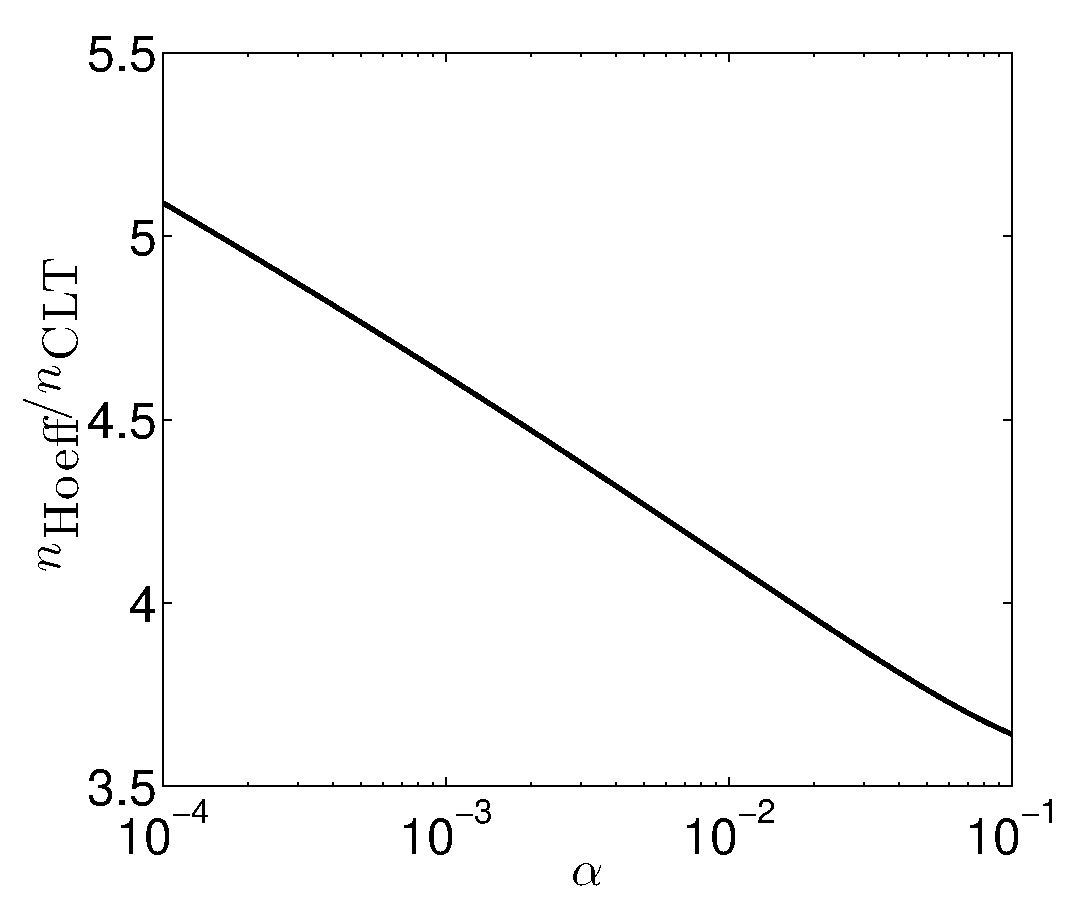
\includegraphics[width=8cm]{plotHoeffCLTr.eps} % requires the graphicx package
    \caption{The computational cost ratio of using Hoeffding's inequality and the CLT to construct a fixed-width confidence interval.}
    \label{fig:ratiovsalpha}
 \end{figure}
\bibliographystyle{alpha}
\bibliography{LJiang}

\end{document}  % end of document